% Claim2Value · 复赛项目说明
% 编译：latexmk -xelatex -interaction=nonstopmode main.tex
\documentclass[11pt,a4paper]{ctexart}

\usepackage[margin=2.2cm,top=2.4cm,bottom=2.2cm,headheight=15pt]{geometry}
\usepackage{xcolor,graphicx,booktabs,array,tabularx,amsmath,amssymb}
\usepackage{tikz}
\usetikzlibrary{arrows.meta,positioning,shapes.geometric,calc,fit,backgrounds}
\usepackage[most]{tcolorbox}
\usepackage{fancyhdr,titlesec,enumitem,fontspec,indentfirst,caption}
\usepackage{pgfplots}
\pgfplotsset{compat=1.18}
\usepackage{hyperref}

% ---------- 品牌色，与产品界面一致 ----------
\definecolor{ink}{HTML}{25272B}
\definecolor{muted}{HTML}{62666B}
\definecolor{line}{HTML}{DEDEDB}
\definecolor{accent}{HTML}{763B32}
\definecolor{accentsoft}{HTML}{C49D95}
\definecolor{track}{HTML}{E8E6E2}
\definecolor{paper}{HTML}{FFFFFF}
\definecolor{softbg}{HTML}{F7F6F4}

% ---------- 字体 ----------
% Noto Sans SC 以可变字体形式安装，按名称调用 Bold 会解析失败，故直接指定文件。
\setCJKmainfont{NotoSansSC-VF.ttf}[Path=C:/Windows/fonts/,BoldFont=NotoSansSC-VF.ttf,AutoFakeBold=1.6]
\setCJKsansfont{NotoSansSC-VF.ttf}[Path=C:/Windows/fonts/,BoldFont=NotoSansSC-VF.ttf,AutoFakeBold=1.6]
\setmainfont{Fira Sans}
\setsansfont{Fira Sans}

\hypersetup{colorlinks=true,linkcolor=accent,urlcolor=accent,citecolor=accent,
            bookmarksnumbered=true,pdftitle={Claim2Value 项目说明},pdfauthor={饮水思源}}

% ---------- 标题层级 ----------
\titleformat{\section}[block]
  {\normalfont\sffamily\bfseries\color{ink}}
  {\fontsize{15}{19}\selectfont\thesection\hspace{0.6em}\textcolor{accent}{\rule[-0.18em]{3pt}{1.15em}}\hspace{0.55em}}
  {0pt}{\fontsize{14.5}{19}\selectfont}
\titlespacing*{\section}{0pt}{16pt}{8pt}
\titleformat{\subsection}{\normalfont\sffamily\bfseries\large\color{ink}}{\thesubsection}{0.6em}{}
\titlespacing*{\subsection}{0pt}{12pt}{5pt}
\titleformat{\subsubsection}{\normalfont\sffamily\bfseries\normalsize\color{accent!85!black}}{\thesubsubsection}{0.6em}{}
\titlespacing*{\subsubsection}{0pt}{9pt}{3pt}

% ---------- 页眉页脚 ----------
\pagestyle{fancy}
\fancyhf{}
\fancyhead[L]{\small\sffamily\color{muted}Claim2Value · 研究工作台}
\fancyhead[R]{\small\sffamily\color{muted}北京大学金融 AI 智能体创新大赛 · 复赛}
\fancyfoot[C]{\small\sffamily\color{muted}\thepage}
\renewcommand{\headrulewidth}{0.4pt}
\renewcommand{\headrule}{\color{line}\hrule width\headwidth height 0.4pt}

\captionsetup{font={small,sf},labelfont={bf,color=accent},labelsep=quad,skip=6pt}

% ---------- 组件 ----------
\newtcolorbox{finding}[1][关键结论]{
  colback=softbg,colframe=accent,boxrule=0.8pt,arc=1.6mm,
  left=10pt,right=10pt,top=7pt,bottom=7pt,
  title={\sffamily\bfseries\small #1},coltitle=white,colbacktitle=accent}
\newtcolorbox{note}[1][说明]{
  colback=white,colframe=line,boxrule=0.7pt,arc=1.6mm,
  left=10pt,right=10pt,top=7pt,bottom=7pt,
  title={\sffamily\bfseries\small #1},coltitle=ink,colbacktitle=track}
\newtcolorbox{codebox}{
  colback=softbg,colframe=line,boxrule=0.6pt,arc=1.2mm,
  left=8pt,right=8pt,top=6pt,bottom=6pt}

\newcommand{\kw}[1]{\textcolor{accent}{\bfseries #1}}
% 代码类文本里含下划线与正则符号，统一走 \detokenize，避免被当成数学或转义。
\newcommand{\code}[1]{\texttt{\small\detokenize{#1}}}
\newcommand{\rawcode}[1]{{\ttfamily\small\detokenize{#1}}}
\setlist[itemize]{leftmargin=1.5em,itemsep=2pt,topsep=3pt,parsep=0pt}
\setlist[enumerate]{leftmargin=1.7em,itemsep=2pt,topsep=3pt,parsep=0pt}

\begin{document}

% =====================================================================
% 封面
% =====================================================================
\thispagestyle{empty}
\vspace*{1.6cm}
{\sffamily\color{muted}\small 北京大学金融 AI 智能体创新大赛 · 复赛}

\vspace{0.5cm}
{\sffamily\bfseries\fontsize{32}{38}\selectfont\color{ink} Claim2Value}

\vspace{0.25cm}
{\sffamily\fontsize{15}{20}\selectfont\color{accent} 面向机器人产业链的财务研究工作台}

\vspace{0.9cm}
\textcolor{accent}{\rule{\textwidth}{1.6pt}}

\vspace{0.7cm}
\begin{tabularx}{\textwidth}{@{}lX@{}}
\toprule
\sffamily\bfseries 团队 & 饮水思源 \\
\sffamily\bfseries 项目 & Claim2Value（研究工作台） \\
\sffamily\bfseries 验证案例 & 绿的谐波（688017）2024 年年度报告，13 页 \\
\sffamily\bfseries 访问方式 & 本地部署包 \code{06_本地部署/}，\code{start_harness.bat}，端口 8510 \\
\sffamily\bfseries 日期 & 2026 年 10 月 12 日 \\
\bottomrule
\end{tabularx}

\vspace{1.0cm}
{\sffamily\bfseries\color{ink} 团队成员与分工}

\vspace{0.3cm}
\begin{tabularx}{\textwidth}{@{}l l X@{}}
\toprule
\sffamily\bfseries 姓名 & \sffamily\bfseries 单位 & \sffamily\bfseries 分工 \\
\midrule
魏孟祺 & 西安交通大学 \, 金禾经济研究中心 & 负责人。项目构建、需求判断与规划 \\
孙圣尧 & 上海交通大学 \, 巴黎卓越工程师学院 & 项目测试、资料搜集与前端优化 \\
陈洛笛 & 西安交通大学 \, 计算机学院 & 代码实现、测试与 review \\
\bottomrule
\end{tabularx}

\vfill
\begin{note}[材料导览]
本文档是复赛作品的主说明，展开信息表中的结论。配套材料：\textbf{\code{03_展示稿}}（快速浏览重点）、\textbf{\code{04_运行视频}}（真实操作过程）、\textbf{\code{05_技术证据}}（可核对的原始记录与输出）、\textbf{\code{06_本地部署}}（可直接启动的产品）。本文档与上述三份材料使用同一组案例和同一组数字。
\end{note}

\clearpage

% =====================================================================
\section{问题与创新}
% =====================================================================

\subsection{要解决的问题}

研究机器人产业链的投资与研究人员，每天面对的是三类材料：企业公告与互动平台答复、券商与产业调研报告、以及上市公司的定期财报。这三类材料的读出方式差别很大，但都会遇到同一个困难：\kw{数字和结论脱离了它们成立的条件，被单独摘出来使用}。

三个真实存在的例子：

\begin{itemize}
  \item \textbf{技术表述省略比较条件。}「减重 30\%」这类说法，如果不说明是否在同等输出扭矩下、与哪一代产品比较、统计口径是全部型号还是某一型号，就无法复核。把这条说法直接写进投资逻辑，等于把未定义的条件当成已确认的事实。
  \item \textbf{财务数字混用报表范围。} 年报的合并报表与母公司报表并列排版，同一指标在两处有不同数值。利润总额、所得税费用、净利润三项尤其容易出现「数值取自母公司表、标注写成合并口径」的错配。这类错误在人工复制粘贴时很难自查，因为它看起来完全正常。
  \item \textbf{单位与期间口径不一致。} 「万台」与「台」、「年度累计」与「单季」、「原版」与「更正后」在原文里往往只相差一两个字，但在建模时是完全不同的量。
\end{itemize}

\begin{note}[案例背景]
本文档所有验证均使用同一份真实原件：\textbf{苏州绿的谐波传动科技股份有限公司（688017）2024 年年度报告}，取自公开披露渠道，共 13 页（第 1、6--7、107--116 页）。选择这份原件的理由是它同时包含第 7 页的主要会计数据摘要与第 107--116 页的完整四张报表，且合并与母公司报表在同一段页码内相邻排版，正好覆盖上述第二类错误。
\end{note}

\subsection{方案的思路}

工作台的整体原则是 \kw{先固定证据，再作判断}。

\begin{center}
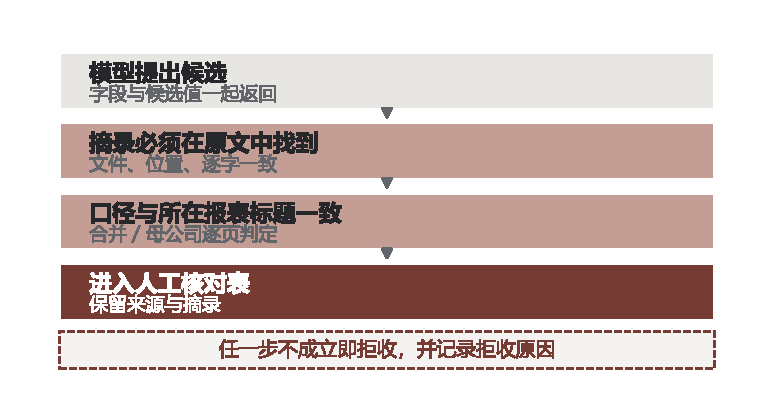
\includegraphics[width=0.86\textwidth]{figures/fig_mechanism.pdf}
\captionof{figure}{财务候选的处理链路。任一环节不成立即拒收，并保留拒收原因。}
\end{center}

财务整理环节要求每一条候选都给出\kw{逐字原文摘录}，并说明这段摘录来自哪个文件的哪一页；代码在原文中检索这段摘录，找不到就直接拒收。通过摘录检查的候选，再核对它声明的报表范围（合并或母公司）是否与所在页面的报表标题一致；不一致的同样拒收。通过这两关之后，还有一道数值与单位必须相连的检查。

观点审查环节走另一条路：把一段企业表述拆成若干条\kw{待检查条件}，在给定材料中分别检索支持证据与反证，并把找不到证据的条件明确列为缺口。规则未覆盖或材料不足时，系统\kw{不作判断}，而不是把缺少反证当作结论成立。

\subsection{方案架构}

\begin{center}
\begin{tikzpicture}[
  font=\sffamily\small,
  node distance=6mm,
  box/.style={draw=line,fill=white,rounded corners=1.4mm,minimum height=9mm,
              inner xsep=7pt,align=center,text=ink},
  rule/.style={draw=accent,fill=softbg,rounded corners=1.4mm,minimum height=9mm,
               inner xsep=7pt,align=center,text=ink},
  svc/.style={draw=line,fill=track,rounded corners=1.4mm,minimum height=8mm,
              inner xsep=7pt,align=center,text=muted},
  ->,>=Stealth,thick,draw=muted
]
\node[box,minimum width=30mm] (src) {原件\\（公告、年报、行情表）};
\node[box,right=14mm of src,minimum width=34mm] (parse) {解析与分片\\页码定位、原文片段};
\node[rule,right=14mm of parse,minimum width=40mm] (engine) {本机规则\\摘录锚定、口径校验、\\单位相邻、时序约束};
\node[box,right=14mm of engine,minimum width=32mm] (out) {人工核对表\\成果与来源记录};

\draw (src) -- (parse);
\draw (parse) -- (engine);
\draw (engine) -- (out);

\node[svc,below=10mm of parse,minimum width=34mm] (model) {自备模型接口\\（提取与检索，按需）};
\draw[dashed] (parse) -- (model);
\node[svc,below=10mm of engine,minimum width=40mm] (local) {本地计算\\核验、盈利变化、回测};
\draw[dashed] (engine) -- (local);
\end{tikzpicture}
\captionof{figure}{三个工作流共用的结构。实线为必经步骤，虚线为按需接入。}
\end{center}

\kw{自研与外部组件的边界}是本项目在架构上刻意区分的一点：

\begin{tabularx}{\textwidth}{@{}lX@{}}
\toprule
\sffamily\bfseries 自研部分 & \sffamily\bfseries 内容 \\
\midrule
证据规则与口径检查 & 摘录锚定、报表标题识别与跨页继承、单位相邻校验、论据分类 \\
记录与留痕 & 运行目录结构、批级进度的断点续取、拒收原因的留存 \\
工程到财务的映射 & 产能、投产、销量、价格、成本参数与估值模型的绑定条件 \\
回测时序 & 信号形成、成交、收益计入的三段错位与费用计算 \\
界面与交互 & 三个工作流的页面、审核步骤与结果呈现 \\
\midrule
\sffamily\bfseries 外部组件 & \sffamily\bfseries 用途 \\
\midrule
大模型接口 & 从原文提取字段候选、按条件检索论据。\textbf{由使用者自备，可完全不用} \\
Streamlit / pandas / NumPy / PyArrow / pypdf & 界面框架、数据处理与 PDF 解析 \\
\bottomrule
\end{tabularx}

需要说明的是，本机规则部分\kw{不调用任何模型}。财务数据核验、数据体检、盈利变化分解与回测都由确定性的本地代码完成，无需密钥，也不产生调用费用。

\subsection{代表性创新}

\subsubsection*{创新一：引用锚定}

模型返回的每一条财务候选都必须携带一段原文摘录。代码检查存在某个原文片段 $p$ 使

\begin{center}
\code{quote} $\subset$ \code{text}$(p)$, \quad
\code{p.source_file} $=$ \code{source_file}, \quad
\code{p.source_locator} $=$ \code{source_locator}
\end{center}

三者同时成立。不成立即拒收，候选序号、声称的字段值与拒收原因一并写入 \code{rejected_candidates.json}，不进入下载包。这条规则把「模型说某个数字是 6,076 万」变成「模型说第 112 页出现了这句话，且这句话在第 112 页确实存在」——前者无法核对，后者可以。

\subsubsection*{创新二：报表口径校验}

报表标题的识别用一条严格的整行匹配：

\begin{codebox}
\rawcode{^[ \textbackslash t]*(合并|母公司)(资产负债表|利润表|现金流量表|所有者权益变动表)[ \textbackslash t]*(（续）)?[ \textbackslash t]*\$}
\end{codebox}

标题必须独占一行，正文里提到这些字样不算标题。随后按页码顺序做\kw{跨页继承}：若本页页首没有新标题，且与上一页页码连续，则沿用上一页最后一个生效的标题。校验时，取出该摘录在整页文本中的\kw{每一次}出现，各自定位到当时生效的标题；只有当所有出现处的标题口径一致、且与候选声明的口径冲突时，才拒收。标题不明或口径无法判定的情形\kw{不作判断}。

\begin{center}

\includegraphics[width=\textwidth]{figures/fig_timing.pdf}
\captionof{figure}{回测时序。信号、成交与收益分别落在三个交易日，避免前视。}
\end{center}

\subsubsection*{创新三：单位相邻校验}

数值与其单位必须在原文中明确相连，用带前置断言的正则检查：

\begin{codebox}
\rawcode{(?<![\textbackslash d.]) 数值 \textbackslash s* 单位}
\end{codebox}

「1 万台」与「1 台」在数字相同的情况下单位不同，换算系数相差 $10^4$。这条检查阻止了把「台」误读成「万台」的候选进入参数。

\subsubsection*{创新四：回测的时序约束}

回测把信号、成交与收益分置三个交易日：T 日收盘后按当日及之前的信息形成信号，T+1 日收盘成交，T+2 日开始计入持仓收益。因子类信号还要求提供带时分与时区的可得时间，超过当日 15:00 的值不参与当日信号，缺失的因子不会被当作零。

\subsubsection*{与常见做法的对照}

\begin{tabularx}{\textwidth}{@{}p{0.26\textwidth}X@{}}
\toprule
\sffamily\bfseries 常见做法 & \sffamily\bfseries 本项目 \\
\midrule
把整份年报交给模型，直接要结论 &
按页与片段切分，每条候选都必须能指回一个具体片段；指不回去的不采纳 \\
\midrule
模型给出的数字直接采信 &
数值必须伴随可在原文中找到的逐字摘录；摘录存在才进入人工核对 \\
\midrule
合并与母公司数据混用后由人工事后检查 &
按页识别报表标题并跨页继承，声明口径与所在标题冲突的候选在生成阶段即拦截 \\
\midrule
只输出最终报告 &
同时输出拒收清单与拒收原因，失败批次保留为缺口，可从断点继续 \\
\bottomrule
\end{tabularx}

% =====================================================================
\section{效果与效率}
% =====================================================================

\subsection{验证安排}

\textbf{样本。}一份真实年报，13 页，包含主要会计数据摘要、合并资产负债表、母公司资产负债表、合并利润表、母公司利润表、合并现金流量表。

\textbf{参照标准。}人工逐页核对的 24 个目标口径，覆盖 12 个指标各两个年度：营业收入、营业成本、归母净利润、利润总额、所得税费用、合并净利润、经营现金流、购建长期资产支付的现金、总资产、总负债、所有者权益、归母权益。参照值全部取自合并报表，逐条标注页码。

\textbf{对照方法。}同一份原件、同一段任务说明、同一个模型接口，前后两轮。第二轮加入报表口径校验，其余条件不变。

\textbf{验证方式。}两轮实测之外，另用\kw{离线复放}做隔离验证：把第一轮已经取到的 32 条候选逐条重新过一遍口径规则，不调用模型。这样可以把「拦截规则本身是否有效」与「模型这一轮碰巧答对」分开。

\subsection{验证结果}

\begin{center}
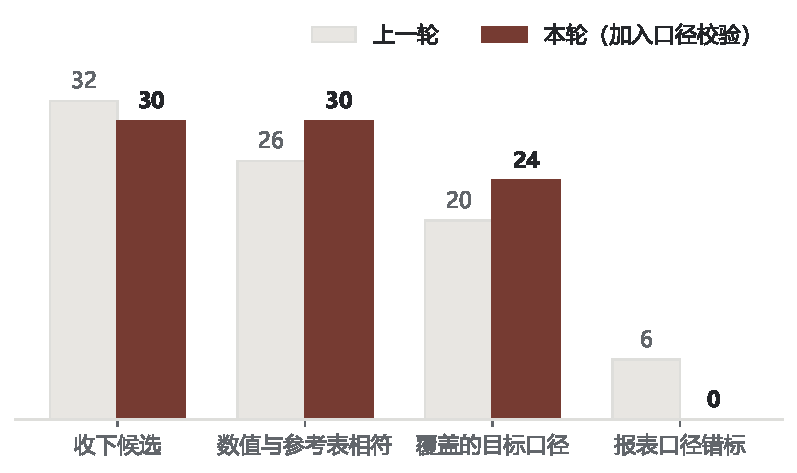
\includegraphics[width=0.94\textwidth]{figures/fig_two_round.pdf}
\captionof{figure}{同一份原件的两轮对比。第二轮加入口径校验，取到的候选数略降，与参照表相符的条数与覆盖的目标口径同时上升。}
\end{center}

\begin{center}
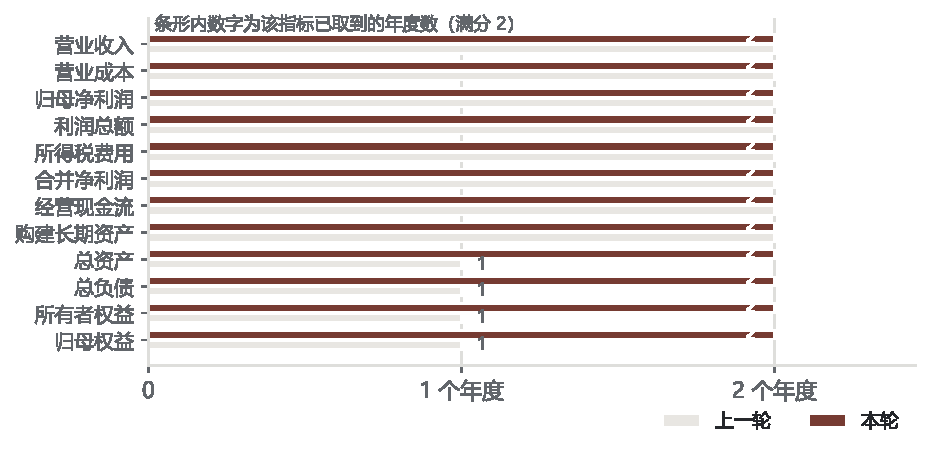
\includegraphics[width=0.94\textwidth]{figures/fig_coverage.pdf}
\captionof{figure}{24 个目标口径的覆盖情况。上一轮在资产、负债与权益四项目标上只取到一个年度，第二轮全部取满两个年度。}
\end{center}

\begin{finding}[第一轮的问题与成因]
第一轮 32 条候选中有 6 条把母公司报表的数字标成了合并口径，分别是 2023 与 2024 两年的利润总额、所得税费用与净利润。

成因已用原件逐页复核：这 6 条数值取自第 114 页，而第 114 页\kw{自身没有报表标题}——「母公司利润表」的标题印在第 113 页页末，单页成批后标题随之丢失，模型因此把第 114 页的数字误认为延续第 112 页的合并利润表。
\end{finding}

\begin{center}
\begin{tabularx}{\textwidth}{@{}l r r l@{}}
\toprule
\sffamily\bfseries 指标 & \sffamily\bfseries 错取值（母公司） & \sffamily\bfseries 参照值（合并） & \sffamily\bfseries 页码 \\
\midrule
利润总额（2024） & 64,572,784.68 & 60,764,068.46 & 第 112 / 114 页 \\
利润总额（2023） & 91,985,161.50 & 91,571,396.66 & 第 112 / 114 页 \\
所得税费用（2024） & 5,525,057.09 & 4,955,333.81 & 第 112 / 114 页 \\
所得税费用（2023） & 9,176,871.02 & 6,739,185.62 & 第 112 / 114 页 \\
净利润（2024） & 59,047,727.59 & 55,808,734.65 & 第 112 / 114 页 \\
净利润（2023） & 82,808,290.48 & 84,832,211.04 & 第 112 / 114 页 \\
\bottomrule
\end{tabularx}
\captionof{table}{第一轮被错标的 6 条候选。金额单位为元。}
\end{center}

\textbf{离线复放的隔离验证。}把第一轮的 32 条候选逐条重放（不调用模型），口径规则\kw{恰好}标出第 23--28 号这 6 条，未误伤其余 26 条。被标出的 6 条没有一条与参照值相符；与参照值不符却漏标的为 0 条。

\begin{finding}[第二轮的实测结果]
加入口径校验后重跑同一份原件：取到 30 条候选，\kw{30 条数值全部与参照表相符}，覆盖 \kw{24 / 24} 个目标口径，报表口径错标 \kw{0} 条，无拒收。

其中 4 个目标口径（资产、负债、权益四项的 2023 年度）是第一轮未取到、第二轮新增的。
\end{finding}

\subsection{典型案例：一次完整的盈利变化分解}

把已核对通过的 24 条记录交给工作台的盈利变化模块，对 2023 与 2024 两个年度做分解。该模块要求两期属于同一公司、同一披露日、同一报表范围、同一修订版本，且两期都必须有收入与成本。

\begin{center}
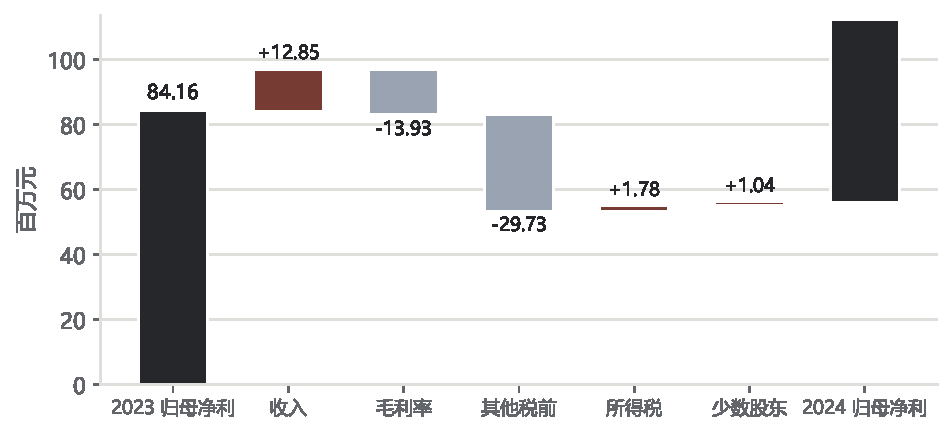
\includegraphics[width=0.94\textwidth]{figures/fig_bridge.pdf}
\captionof{figure}{归母净利润变化分解。各项贡献之和与目标变化完全相等，残差为 0。}
\end{center}

\begin{center}
\begin{tabularx}{\textwidth}{@{}X r l@{}}
\toprule
\sffamily\bfseries 分解项 & \sffamily\bfseries 贡献（元） & \sffamily\bfseries 计算方式 \\
\midrule
收入变化贡献 & $+12{,}853{,}079.74$ & $(R_1-R_0)\,m_0$ \\
毛利率变化贡献 & $-13{,}930{,}083.80$ & $R_1\,(m_1-m_0)$ \\
其余税前项目净变化 & $-29{,}730{,}324.14$ & $(P_1-GP_1)-(P_0-GP_0)$ \\
所得税费用变化 & $+1{,}783{,}851.81$ & $-(T_1-T_0)$ \\
少数股东损益变化 & $+1{,}036{,}308.50$ & $-[(NP_1-NPP_1)-(NP_0-NPP_0)]$ \\
\midrule
\textbf{合计} & $\mathbf{-27{,}987{,}167.89}$ & 与归母净利润实际变化一致，残差 0.00 \\
\bottomrule
\end{tabularx}
\captionof{table}{归母净利润桥。$R$ 为营业收入，$m$ 为毛利率，$GP$ 为毛利，$P$ 为利润总额，$T$ 为所得税费用，$NP$ 为合并净利润，$NPP$ 为归母净利润。}
\end{center}

营业收入同比增加 8.77\%，但毛利率从 41.14\% 降至 37.54\%，使毛利率变化贡献为 $-1{,}393$ 万元，抵消并超过收入增长带来的 $+1{,}285$ 万元；其余税前项目净减少 $2{,}973$ 万元，是归母净利润下降 $2{,}799$ 万元的主要来源。

\begin{note}[对这条分解的说明]
输出中的所有数值都可以按页码回溯到原件：收入与营业成本来自第 7 页与第 112 页，利润总额、所得税费用与合并净利润来自第 112 页，归母净利润来自第 113 页。分解是\kw{会计恒等式的重排}，不是因果识别；「其余税前项目」合并了费用、投资收益与减值等的净影响，不能据此推断某一项技术进展带来了多少利润。经营现金流减购建长期资产支出只是现金差额，未经调整不构成估值用的自由现金流。
\end{note}

\subsection{效率与成本}

\begin{center}
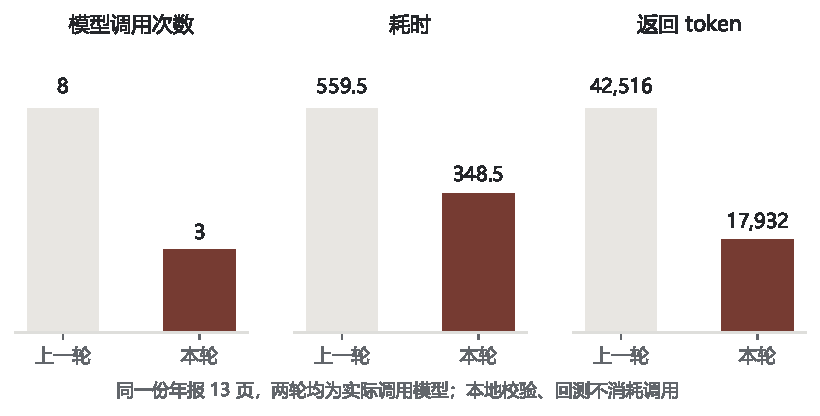
\includegraphics[width=0.94\textwidth]{figures/fig_efficiency.pdf}
\captionof{figure}{两轮实测的调用次数、耗时与返回 token。}
\end{center}

\begin{center}
\begin{tabularx}{\textwidth}{@{}X r r@{}}
\toprule
\sffamily\bfseries 指标 & \sffamily\bfseries 第一轮 & \sffamily\bfseries 第二轮 \\
\midrule
模型调用次数 & 8 次 & 3 次 \\
端到端耗时 & 559.5 秒 & 348.5 秒 \\
返回 token & 42,516 & 17,932 \\
输入 token & 16,817 & 9,153 \\
与参照表相符 & 26 / 32 & 30 / 30 \\
覆盖目标口径 & 20 / 24 & 24 / 24 \\
\midrule
本地计算调用次数 & \multicolumn{2}{c}{0 次（核验、盈利变化、回测均不调用模型）} \\
\bottomrule
\end{tabularx}
\end{center}

第二轮把年报 13 页切成 2 批，单批上限 6000 字符，两批分别 5693 与 5680 字符。第一批的首次请求遇到网络中断，等待 143.6 秒后失败，按重试策略等待 1 秒后重发，95.5 秒完成；第二批一次完成，108.3 秒。

耗时下降主要来自批数减少：第一轮的 8 次调用中有 6 次是上下文超限后的切分重试，第二轮因为改进了分片策略，两批即完成。费用按使用者所选服务商的实际计价结算，本项目不代收、不抽成。

\begin{finding}[可复现的工程检查]
工作台自带 \textbf{557 项}自动化测试，全部通过；另有 2 项因 Windows 符号链接权限跳过。测试覆盖摘录锚定、口径校验、断点续取、预算与额度中断、密钥不落盘、成果包不含原件等行为。
\end{finding}

% =====================================================================
\section{适用性与呈现}
% =====================================================================

\subsection{访问与操作}

\begin{center}
\begin{tabularx}{\textwidth}{@{}lX@{}}
\toprule
\sffamily\bfseries 项目 & \sffamily\bfseries 说明 \\
\midrule
访问方式 & 本地部署包，目录 \code{06_本地部署/} \\
启动命令 & Windows 双击 \code{start_harness.bat}；Linux 执行 \code{bash start_harness.sh} \\
默认账号 & 无需登录 \\
浏览器地址 & \code{http://127.0.0.1:8510} \\
环境要求 & Python 3.12；首次安装依赖需联网，约 500 MB \\
密钥 & 本地计算不需密钥。仅提取与检索需自备模型接口，密钥只留在当前浏览器会话 \\
\bottomrule
\end{tabularx}
\end{center}

\kw{典型操作路径}（与运行视频的分段一致）：

\begin{enumerate}
  \item \textbf{财务整理。}选择「整理财务数据」，上传年报并指定页码范围，或直接导入已整理的 16 列财务长表。前者由模型分批提取候选，后者完全本地校验。
  \item \textbf{核对与校验。}对照原件检查候选的 16 个字段，补齐实际披露日、单位与修订版本，勾选确认后执行校验。未采用候选与拒收原因在页面上单独列出。
  \item \textbf{生成成果。}校验通过后生成标准化结果、质量标准、历史比率与 Excel；字段齐备时可继续生成两期盈利变化与可选的 DCF 敏感性。
  \item \textbf{观点审查。}把企业表述拆成待检查条件，在给定材料中检索支持与反证，列出缺口。模型不可用时可用本地模板编辑条件。
  \item \textbf{策略回测。}先做数据体检（列映射、代码格式、日期、重复、缺失与因子可得时间），再运行回测，得到净值、回撤、费用与同费率基准；可预先声明参数组做对照诊断。
\end{enumerate}

\subsection{稳定性与异常处理}

\begin{tabularx}{\textwidth}{@{}lX@{}}
\toprule
\sffamily\bfseries 情形 & \sffamily\bfseries 处理方式 \\
\midrule
单批失败 & 该批保留为缺口，其余批次继续；再次点击只请求未完成的部分 \\
上下文超限或输出截断 & 按片段自动拆小后重试，最多四层；仍失败的范围留为缺口 \\
网络中断或临时服务错误 & 有限次重试并记录每次尝试；认证、硬额度与预算问题直接停止 \\
预算耗尽 & 停止后续请求，已完成批次的结果保留可查 \\
文件无法读取 & 在处理前列出问题文件，不让整个流程静默失败 \\
浏览器会话结束 & 原件与结果保留在本机运行目录；当前版本不提供跨会话继续按钮 \\
\bottomrule
\end{tabularx}

\subsection{人工环节}

以下几处\kw{必须由人确认}，系统不代替判断：

\begin{itemize}
  \item 候选字段的映射是否正确。摘录存在只说明这段话在原文里，不说明它被放进了正确的字段。
  \item 数据缺口是否接受。缺披露日 14 条、缺修订标记 30 条、缺股票代码 16 条、6 组重复记录需要人工取舍——这些缺口会被明确列出，但不会被自动填上猜测值。
  \item 估值参数是否是用户自己的假设。五年自由现金流、折现率与永续增长率来自使用者填写，不从历史报表或模型意见自动升级为预测。
  \item 观点审查的结果如何使用。检索覆盖有范围限制，找不到证据的条件被列为缺口，而不是判定为不成立。
\end{itemize}

\subsection{适用边界与迁移条件}

\textbf{当前适用范围。}上市公司定期报告与公告的财务数据核对，以及公开材料的论据检索。三个工作流都以中文文本与 A 股口径为主。

\textbf{明确的限制。}扫描件不含 OCR，需先自行转换；无可识别报表标题的页面不作口径判断；多指标混排的复杂表格仍以人工核对为准；回测未模拟停牌、上市退出、涨跌停、冲击成本与成交量约束；已查看过的区间不构成未触碰的留出集。

\textbf{迁移到其他公司或行业}需要补齐三件事：原件与字段定义（不同公司披露格式不同）、参数口径审核（产能、单价、成本需要各自的定义）、以及该行业的可比公司参照。这三项都是配置工作，不涉及模型重训。

\textbf{平台验证。}Windows 11 已完成一键启动与实际操作验收；Linux 提供同一套启动脚本，未在真机验证。

% =====================================================================
\section{初赛后的深化}
% =====================================================================

\begin{tabularx}{\textwidth}{@{}p{0.22\textwidth} X X@{}}
\toprule
\sffamily\bfseries 方面 & \sffamily\bfseries 初赛状态 & \sffamily\bfseries 本次深化 \\
\midrule
产品形态 &
固定案例的演示程序，数据与结论预先置入 &
可上传自备文件的研究工作台，三个工作流，本地部署可启动 \\
\midrule
财务提取 &
模型返回字段，人工核对后使用 &
加入逐字引用锚定与报表口径校验；未采用的候选与原因一并展示 \\
\midrule
验证方式 &
单轮人工抽查 &
同一原件的两轮实测对照，外加离线复放做隔离验证；24 个目标口径逐条比对 \\
\midrule
数据体检 &
无 &
回测前先检查列映射、代码格式、日期、重复、缺失与因子可得时间 \\
\midrule
运行记录 &
过程不落盘 &
运行目录记录原件、中间状态与拒收原因；批级进度支持断点续取 \\
\midrule
边界说明 &
较少 &
在界面上标明本地计算与外部调用的分界，明确列出需要人工确认的环节 \\
\bottomrule
\end{tabularx}

% =====================================================================
\section{局限与下一步}
% =====================================================================

\textbf{已知局限。}验证集中在一家公司的一份年报上，样本量小；口径校验依赖报表标题的整行文本，对图片型或特殊排版的报表无效；单位校验目前覆盖产能、订单与价格三类参数，未覆盖全部财务指标；检索为词法匹配，不具备完整的语义理解能力；扫描件需要先做 OCR；模型提取的质量与所选服务商的能力有关，更换模型后需要重新核验。

\textbf{下一步计划。}第一，把案例集扩展到不同行业与不同披露格式，用同一套规则复现，识别规则失效的边界。第二，把单位与口径校验的覆盖面从当前三类参数扩展到全部财务指标。第三，补齐数据库字段的正式定义与枚举，使外部数据可以按同样的严格度接入。第四，在产品页面内做逐条件的进度提示，减少长任务的等待不确定性。

\vspace{0.8cm}
\begin{note}[关于本文档中的数字]
本文档、展示稿、运行视频与技术证据目录使用同一组数字。全部原始收据（两轮实测记录、离线复放记录、部署与录屏验收记录）见 \code{05_技术证据/}，每份收据都带文件哈希，可逐条核对。
\end{note}

\clearpage

% =====================================================================
\appendix
\renewcommand{\thesection}{附录 \Alph{section}}
\section{财务长表的 16 个字段}

\begin{center}
\begin{tabularx}{\textwidth}{@{}l l X@{}}
\toprule
\sffamily\bfseries 字段 & \sffamily\bfseries 含义 & \sffamily\bfseries 校验要点 \\
\midrule
\code{stock_code} & 股票代码 & 六位文本，保留前导零 \\
\code{company} & 公司名称 & 必填 \\
\code{report_period} & 报告期 & 有效日期 \\
\code{published_at} & 实际披露日 & 期末日 $\le$ 披露日 $\le$ 研究截止日 \\
\code{statement_scope} & 报表范围 & 仅 \code{consolidated} 或 \code{parent} \\
\code{period_type} & 期间口径 & 时点值须为 \code{point_in_time}；流量须区分年度、累计与单季 \\
\code{metric_original} & 原指标名 & 必填 \\
\code{canonical_metric} & 标准指标 & 须在支持列表内 \\
\code{value_original} & 原值 & 可解析为有限数值 \\
\code{unit} & 单位 & 元、万元、亿元之一 \\
\code{currency} & 币种 & 仅 \code{CNY} \\
\code{revision_flag} & 修订版本 & 必填，区分原版与更正 \\
\code{source_database} & 来源 & 必填 \\
\code{source_file} & 原件文件名 & 相对路径，须存在于运行目录 \\
\code{source_locator} & 原文位置 & 页码或段落定位 \\
\code{source_sha256} & 原件指纹 & 与上传字节一致 \\
\bottomrule
\end{tabularx}
\end{center}

组级校验另有三项：同一分组内同一指标与期间口径不得重复；资产负债表的资产等于负债加所有者权益，容差 1 元；毛利率按 $(R-C)/R$ 计算但不判定对错。

\section{校验错误码}

\begin{center}
\begin{tabularx}{\textwidth}{@{}l X@{}}
\toprule
\sffamily\bfseries 错误码 & \sffamily\bfseries 界面提示 \\
\midrule
\code{stock_code_requires_six_digits} & 股票代码须保留六位文本。回到源数据恢复前导零，不猜测代码。 \\
\code{publication_or_period_after_cutoff} & 报告期、实际披露日和截止日的先后关系无效。核对实际日期或调整研究范围，不倒填日期。 \\
\code{unknown_statement_scope} & 报表范围须区分合并与母公司，按模板选择。 \\
\code{unknown_canonical_metric} & 标准指标不受支持，请对照财务模板映射原指标，不猜口径。 \\
\code{stock_metric_requires_point_in_time} & 资产、负债、权益等时点值须选时点口径，不作累计或年度流量。 \\
\code{invalid_flow_period_type} & 收入与利润等流量须区分年度、累计和单季。 \\
\code{annual_flow_requires_december_31} & 年度流量须对应 12 月 31 日期末；中期流量保留中期口径。 \\
\code{unsupported_unit_or_currency} & 核对金额单位与币种。仅使用模板支持的单位，不混用万元、亿元。 \\
\code{source_file_missing} & 对应原件没有上传。请上传原件并核对财务长表的文件名。 \\
\code{source_hash_mismatch} & 原件指纹不匹配。核对是否上传了不同版本，不直接改指纹绕过检查。 \\
\code{duplicate_metric_requires_review} & 同口径指标重复。检查更正版本及重复行，再人工决定保留哪条。 \\
\code{balance_sheet_mismatch} & 资产负债表不平衡。核对资产、负债、权益是否同期间、同版本、同报表范围。 \\
\code{invalid_number} & 原始数值不能解析。核对数字与单位，缺失值不填零。 \\
\code{nonfinite_number} & 数值不能是无穷大或 NaN。回到原件核对，缺失值保留为空。 \\
\bottomrule
\end{tabularx}
\captionof{table}{每条错误都附中文说明与处理方向，而不是只给一个代号。}
\end{center}

\section{依赖与运行环境}

\begin{center}
\begin{tabularx}{\textwidth}{@{}l l X@{}}
\toprule
\sffamily\bfseries 组件 & \sffamily\bfseries 版本 & \sffamily\bfseries 用途 \\
\midrule
Python & 3.12 & 运行环境 \\
Streamlit & 1.64.0 & 本地界面 \\
pandas & 2.2.3 & 数据处理 \\
NumPy & 2.3.5 & 数值计算 \\
PyArrow & 20.0.0 & 列式数据读写 \\
openpyxl & 3.1.5 & Excel 输出 \\
pypdf & 6.10.0 & PDF 文本与页码定位 \\
\bottomrule
\end{tabularx}
\end{center}

以上为直接依赖，版本固定于 \code{requirements-harness.txt}，间接依赖由 pip 解析。首次安装需要联网，之后本地计算不依赖网络。

\end{document}
